\chapter{WiFi Offloading}
\label{chap:offloading}

\section{Background}\label{background}
With the advent of the smartphone, mobile data usage has exploded which in turn has created tremendous pressure on cellular data networks.  A promising candidate to reduce the impact of cellular data growth is WiFi offloading. However, our dataset casts doubts on the viability of achieving such 
gains with WiFi offloading. In contrast to the prior work of \cite{lee2010mobile}, we have found that despite users operating in a dense university WiFi environment, the potential gains for the majority of users are quite muted. Rather than finding that WiFi usage dominates 3G usage, our study curiously finds that much of the user consumption of 3G dominates the consumption of WiFi. 

At first glance, such a result would appear to counterintuitive. A dense WiFi deployment\footnote{The
University of Notre Dame was ranked as one of the top 20 wireless campuses in 2010.} would have ample
WiFi access points placed throughout the buildings on the campus. The dormitory-oriented residential
life of the campus meant that all study participants (all of whom were freshmen) would have ubiquitous
WiFi coverage at night (dormitory) as well as during the day (classrooms/dorms). Coverage at the
university is also frequently verified by employing roaming laptops by IT staff throughout campus. However, it is the usage of laptops to validate coverage as opposed to smartphones where the problem
originates.

Consider the observation noted in Table~\ref{table:diff_rssi} that compares the observed RSSI on 
a laptop versus the RSSI observed in the same time period and same location via a representative smartphone 
from the study. In the table, despite being in the same location, the smartphone observes a dramatically
reduced signal strength (around 10dB) versus the laptop. The discrepancy between observed signal strength on the smartphone
is not an isolated phenomenon to one particular smartphone but rather tends to be broadly indicative of many
commercially available smartphones that are subject to marketing and development constraints. This is 
potentially significant for WiFi offloading as most dense WiFi environments (i.e. businesses) tend not 
to be designed at smartphones but rather tend to be designed at laptops.  

\begin{table}[h!tbp] 
\caption{WIFI RSSI ON LAPTOP AND SMARTPHONE} 
\label{table:diff_rssi}
\centering 
\begin{tabular}{|c|c|c|c|c|}
\hline
& \multicolumn{2}{c|}{RSSI on Laptop} & \multicolumn{2}{c|}{RSSI on Smartphone} \\
\hline Access Point & Avg. & Std Dev & Avg. & Std Dev \\
\hline 1 & -75.27 & 2.76 & -83.32 & 2.72  \\ 
\hline 2 & -75.22 & 2.79 & -85.04 & 3.39 \\
\hline 3 & -75.40 & 2.87 & -84.94 & 3.04\\
\hline 4 & -71.99 & 2.06 & -79.52 & 3.51\\
\hline 5 & -72.05 & 2.06 & -80.18 & 3.80\\
\hline 6 & -73.88 & 5.13 & -80.02 & 3.34\\
\hline
\end{tabular}
\end{table}

The period in question analyzed in
this chapter represents eight weeks of continuous data from the end of January 2012 to the end of March of 2012 in the spring semester. The time frame is selected to ensure that the students have fully adapted to 
their phones and represent behaviors typical of their normal phone usage.  The seventh week in the study 
represents spring break (March 10th - March 18th) which offers a likely period where students returned home
for the week. In total, we selected 131 users out of the study (62 female, 69 male) that have continuous data throughout the
entire eight weeks and have more than five minutes per day of usage on the phone. The graphs and tables in this chapter are based on the data collected from these 131 participants. 

\section{Related work}\label{related}
There have been several recent studies proposed to reducing the strain on the overloaded cellular infrastructure with WiFi offloading being one of the main candidate~\cite{balasubramanian2010augmenting,lee2010mobile,dimatteo2011cellular,icc2012performance,han2011mobile}. In~\cite{balasubramanian2010augmenting}, WiFi connectivity is used to reduce the pressure on 3G spectrum when possible for transferring data. In~\cite{lee2010mobile,dimatteo2011cellular,icc2012performance,han2011mobile}, delayed WiFi offloading is introduced to migrate data traffic from cellular networks to WiFi access points. However, such methods are not practical for most access patterns (any interactive app including web browsing and most streaming) as the point of using the smartphone is for data access that moment. Conversely, the de facto solution is upgrading the network to the next generation networks. The configuration details of both WiMAX and LTE technologies are summarized in \cite{khan20094g}. Similarly, \cite{arshad2010evolution} provided an overview of the 4G evolution and categorized how such technologies can accompany a more user focused world of wireless. 

\section{WiFi Offloading in Practice}
Figure~\ref{fig:avg_downlink} shows the average 3G and WiFi downlink traffic per phone per week across the study period. On average, the WiFi traffic takes approximately 30\% of the total data consumption. The average WiFi traffic statistics excludes the data of devices with no WiFi usage. The underlying 802.1X WiFi infrastructure (primarily due to expired passwords) can prevent a user from using any WiFi traffic during that entire week. Once the password is updated (passwords are required to change every 90 days), the phone can correctly use WiFi once again. We note though that an inability to authenticate does not preclude monitoring signal strength (via beacons) and that users do not experience intermittent 802.1X issues (the phones either authenticate or do not contiguously).   

\begin{figure}[h!tbp]
\centering
{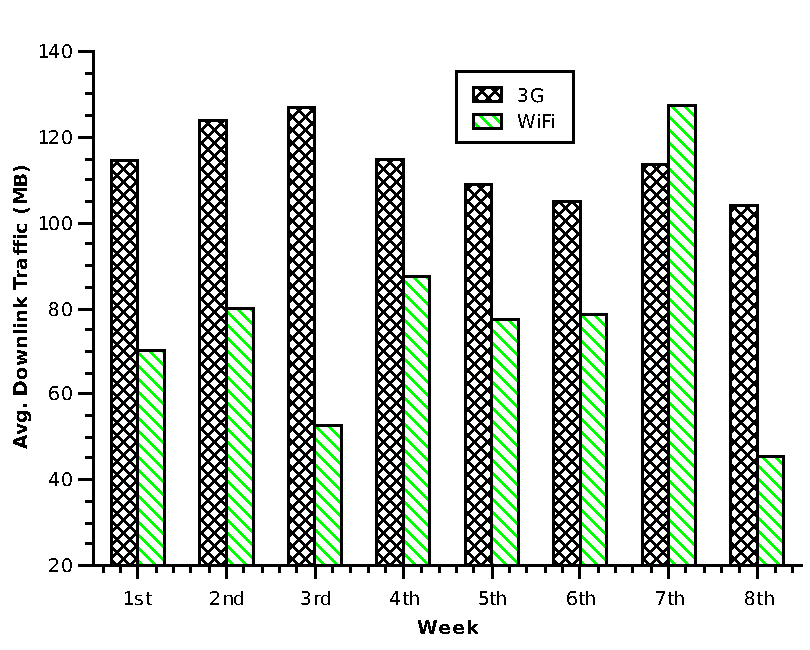
\includegraphics[width = 3.5in]{graphs/avg_downlink2.pdf}}
\caption{Average Downlink Traffic per Phone per Week} 
\label{fig:avg_downlink}
\end{figure}

As noted in Section~\ref{background}, the average WiFi usage is curiously lower than the average 3G usage aside from the week of spring break (likely on a single AP at home) where WiFi barely eclipses 3G usage. In Figure~\ref{fig:switch}, we select a small subset of phones that exhibit a high degree of 3G usage versus WiFi and plot their respective average traffic patterns for a given day during the semester. From 5 PM to 6 PM (1700-1800h), the phones exhibit a degree of asymmetry, favoring 3G over WiFi.  Figure~\ref{fig:weak_wifi_68} explores this time period further noting the detected AP beacons but exceptionally low quality signal strengths over that time period. Hence, the phone naturally defaults to favor 3G over WiFi.  Conversely, during the 10 PM to 11PM (2200-2300h) as noted in Figure \ref{fig:weak_wifi_1012} where the signal strength is better but not great, the ratio between 3G and WiFi changes to favor WiFi over 3G but not markedly so.   

\begin{figure}[h!tbp]
\centering
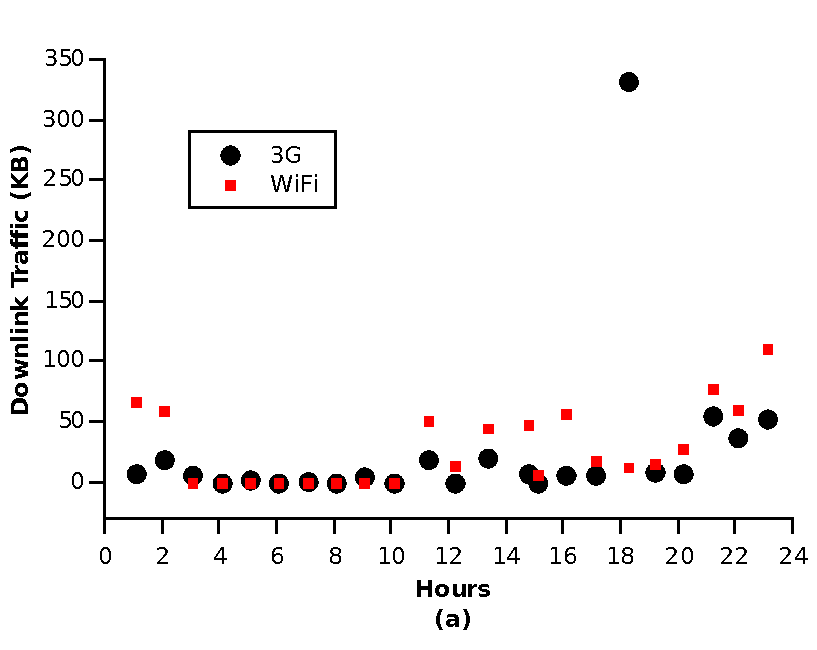
\includegraphics[width = 3.5in]{graphs/traffic_0202.pdf}
\caption{Switch between 3G and WiFi} 
\label{fig:switch}
\end{figure}

\begin{figure}[h!tbp]
\centering
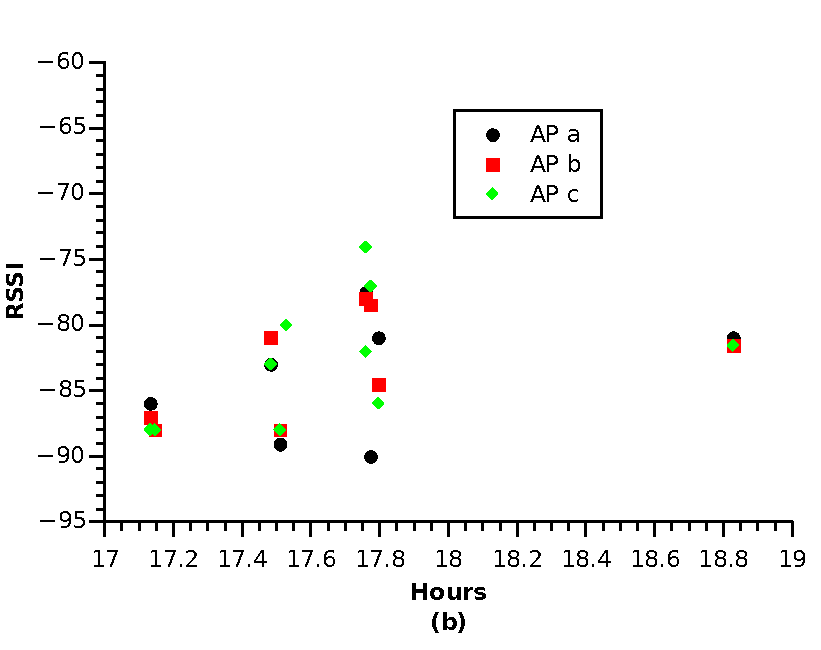
\includegraphics[width = 3.5in]{graphs/weak_wifi_68.pdf}
\caption{WiFi Signal Strength (1700-1800h)} 
\label{fig:weak_wifi_68}
\end{figure}

\begin{figure}[h!tbp]
\centering
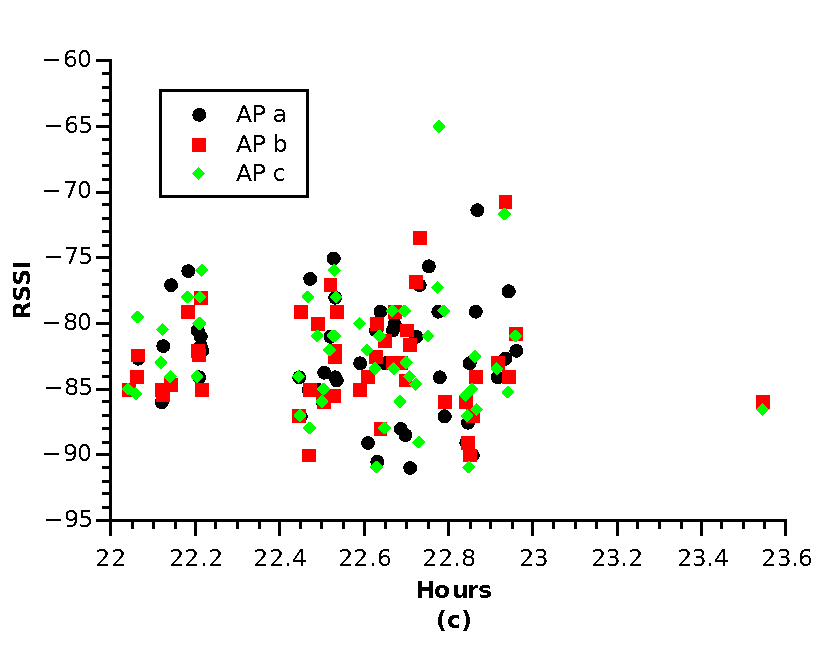
\includegraphics[width = 3.5in]{graphs/weak_wifi_1012.pdf}
\caption{WiFi Signal Strength (2200-2300h)} 
\label{fig:weak_wifi_1012}
\end{figure}

To verify that the users in this subset were indeed active (using the screen), Figure \ref{fig:screen_0202} plots the average screen session lengths over that same selected day. The screen session time captures via event when the screen is turned on (timestamp recorded) and when the screen is turned off (timestamp recorded). While the users were more active in terms of the number of sessions during the later time period (10PM to midnight), the users actually used more data during the earlier time period. We also note that the spike did not correlate with a check in by the agent as such data has been filtered from the results.   

\begin{figure}[h!tbp]
\centering
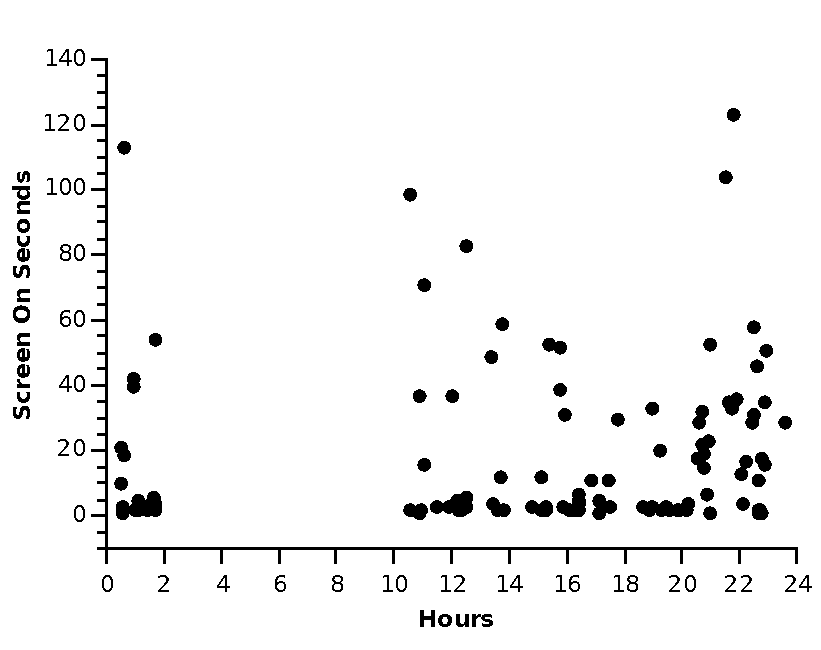
\includegraphics[width = 3in]{graphs/screen_0202.pdf}
\caption{Screen On Duration in One Day} 
\label{fig:screen_0202}
\end{figure}

\section{Comparison of User Behavior}\label{comparison}
We continue our analysis by exploring how user behavior changes if the user is able to get reasonable quantities of 
adequate WiFi smartphone coverage. Figure~\ref{fig:distribution} shows the distribution of the percentage of WiFi downlink
traffic as a ratio versus total traffic for one week (2nd week). The average WiFi consumption ratio is around 30\%. From the figure, we see that there are approximately 30\% of participants whose traffic is offloaded to WiFi for the week by more than 50\%. Conversely, we see that there are 
nearly 20\% of the participants that week who used no WiFi traffic for the reasons mentioned earlier (incorrect password, etc.).

\begin{figure}[h!tbp]
\centering
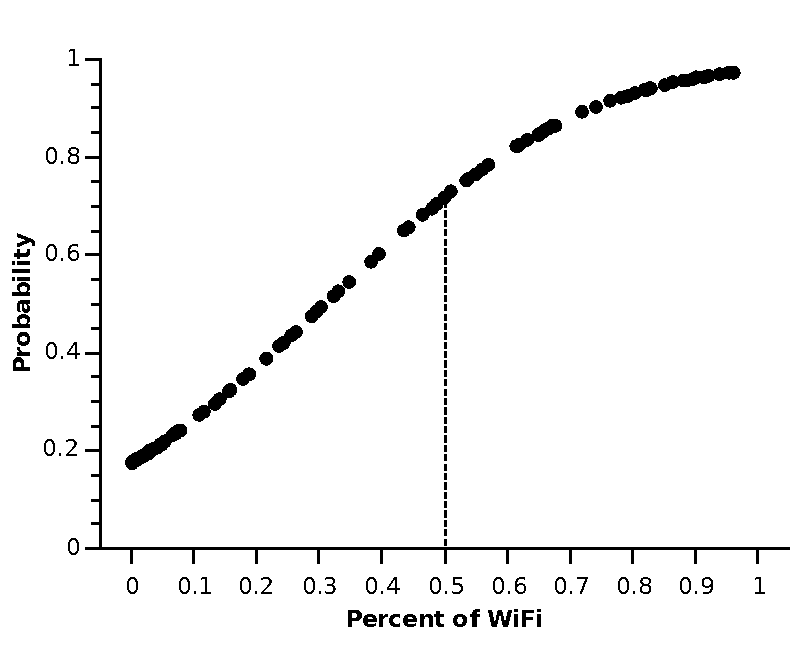
\includegraphics[width = 3.5in]{graphs/distribution.pdf}
\caption{Distribution of Percent of WiFi Traffic} 
\label{fig:distribution}
\end{figure}

For further analysis in the paper, we subdivide the 131 participants into three groups based on their WiFi downlink consumption
ratio versus their total traffic consumption: no WiFi, less than 50\%, and more than 50\%.  We summarize how the participants
break down into each group among the eight weeks in Figure~\ref{fig:number}.  Similarly, the breakdown of males versus females
is shown in Table~\ref{table:gender}. Although the numbers in the  
groups varied, the groups are reasonably well separated to analyze the participants in the various categories.  

\begin{figure}[h!tbp]
\centering
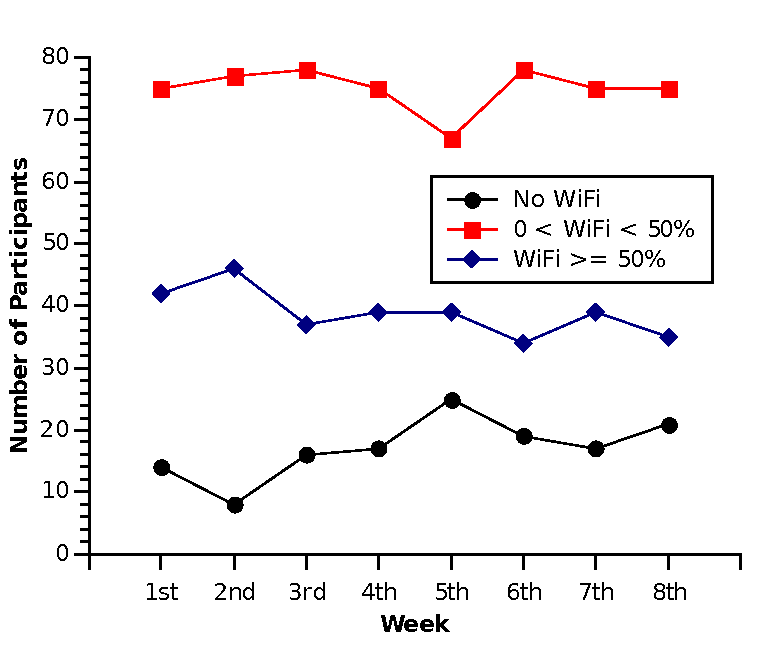
\includegraphics[width = 3.5in]{graphs/number.pdf}
\caption{Numbers of Participant in Groups} 
\label{fig:number}
\end{figure}

\begin{table}[h!tbp] 
\caption{NUMBER OF MALES AND FEMALES IN GROUPS} 
\label{table:gender}
\centering 
\begin{tabular}{|c|cc|cc|cc|}
\hline
Week &  \multicolumn{2}{c}{No WiFi} & \multicolumn{2}{|c|}{0 $<$ WiFi $<$ 50\%} & \multicolumn{2}{c|}{WiFi $>=$ 50\%} \\
\hline
& M & F & M & F &   M & F \\
\hline
 \parbox[t]{3cm}{\hspace{12mm}1st}& 9&5&35&40&25&17\\ 
\hline
2nd &6&2	&35&42&29&17\\
\hline
3rd&5&11&37&41&27&10\\
\hline
4th&7&10&36&39&26&13\\
\hline
5th&15&10&30&37&24&15\\
\hline
6th&9&10&39&39&21&13\\
\hline
7th&8&9&36&39&25	&14\\
\hline
8th&10&11&36&39&23&12\\
\hline
\end{tabular}
\end{table}

Figure~\ref{fig:downlink} shows the average total downlink traffic per phone (3G+WiFi) of the different groups across the eight weeks. For the category of each particular participant, determination was computed on a weekly basis meaning that a user could move between categories. Interestingly enough, we begin to see a growing pattern of separation as the semester goes on and particularly so doing the week of spring 
break. We posit that the week of spring break offered a much more consistent set of WiFi coverage versus what may occur on campus.   

\begin{figure}[h!tbp]
\centering
{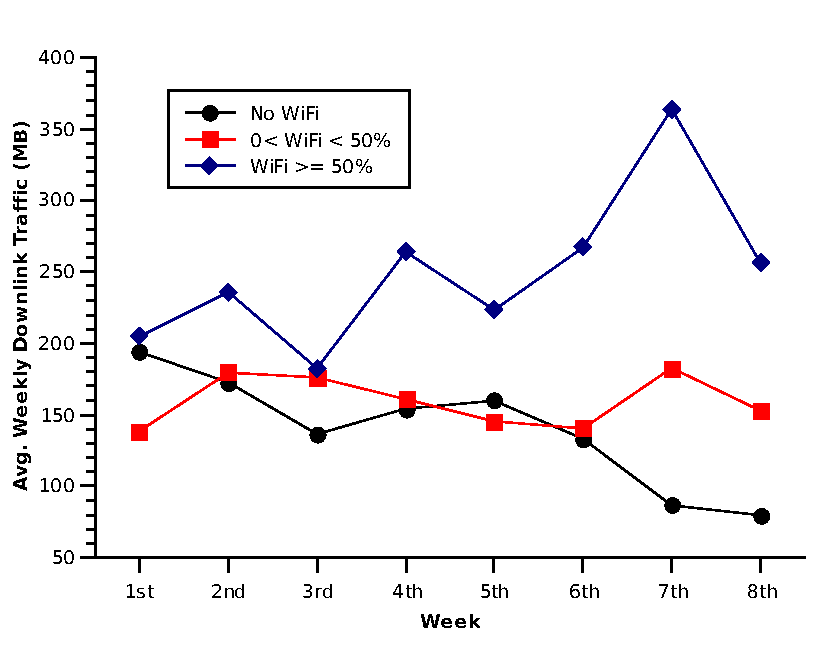
\includegraphics[width = 3.5in]{graphs/downlink.pdf}}
\caption{Weekly Average Total Downlink Traffic per Phone} 
\label{fig:downlink}
\end{figure}

\subsection{Phone Usage}
Related to usage, a secondary question arises with regards to the ratio of screen time to data consumption.  The most straightforward way to indicate whether the person is using the phone is based on the phone screen status (on or off). When the phone screen is on, it is most likely because the person is actively using the phone (sending messages, checking e-mail, playing games, etc.). In order to explore the relationship between phone usage time and traffic usage, we collect the screen on session length on the phones by calculating the duration between screen on and screen off. On average, the screen session lengths vary from 10 seconds to more than 100 seconds. We categorize them into four ranges: (0, 30s), (30s, 60s), (60s, 90s) and more than 90s. Figure~\ref{fig:duration} lists the numbers of participants from three groups in different duration ranges. In the range of (60s, 90s) the number of people who use WiFi more than 50\% is greater than the other two groups numbers. We calculate the weekly total screen on time and the corresponding daily average per phone as well. There are five ranges of daily average from less than half an hour per day to more than 2 hours per day. Figure~\ref{fig:screen} gives an example (data from the 2nd week): compared with purely 3G users (no WiFi), the number of participants who use WiFi more than 50\% in each range is much greater.  The fact that the phone is more useful (faster access) may encourage such additional usage. 

\begin{figure}[h!tbp]
\centering
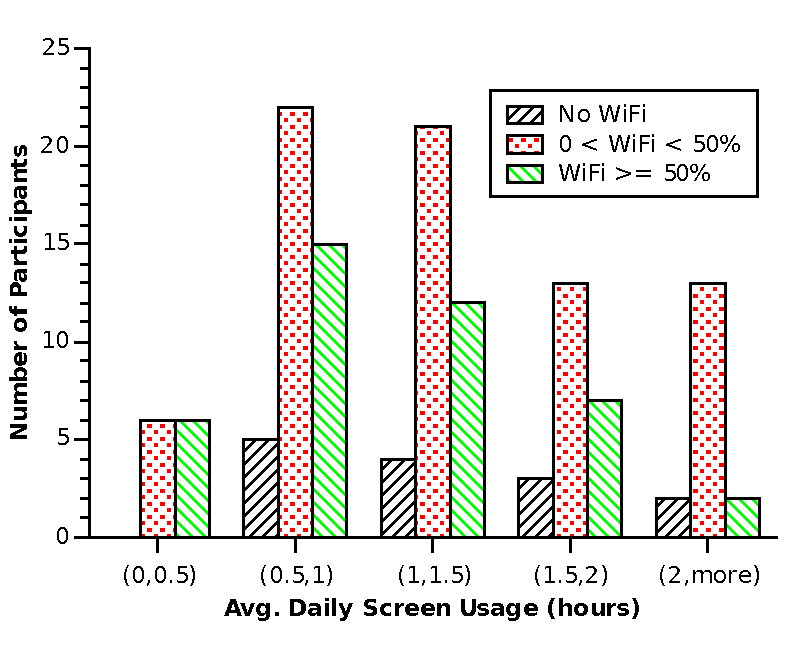
\includegraphics[width = 3.5in]{graphs/screen2.pdf}
\caption{Avg. Daily Screen Usage of Groups} 
\label{fig:screen}
\end{figure}

\begin{figure}[h!tbp]
\centering
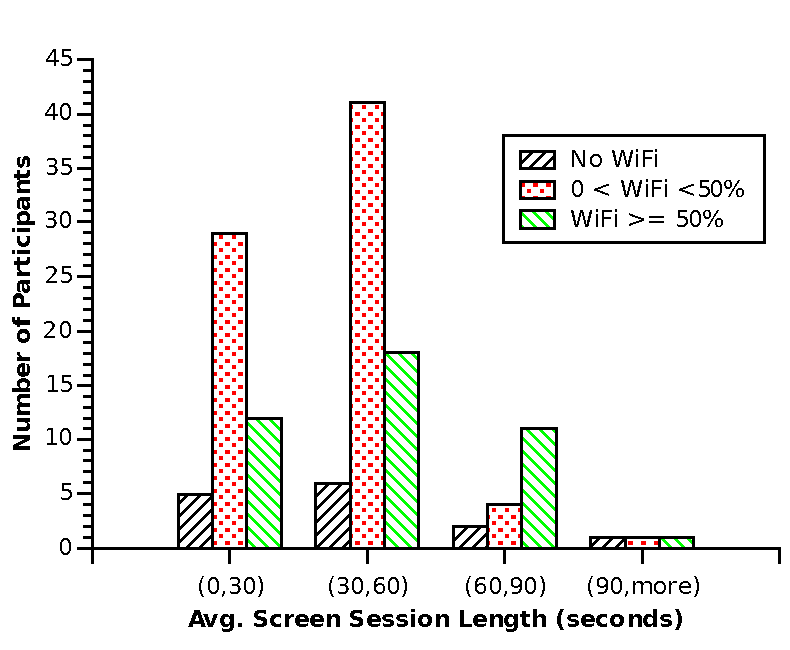
\includegraphics[width = 3.5in]{graphs/duration2.pdf}
\caption{Avg. Screen session length of Groups} 
\label{fig:duration}
\end{figure}

We further calculate the screen session duration across different time slots in a single day to analyze user behavior. As shown in Figure~\ref{fig:dn}, we divide one day into four time slots: morning (7am-12pm), afternoon (12pm-5pm), night (5pm-10pm) and midnight (10pm-7am).  As would
be expected with a student population, usage in the morning is quite low relative to usage in the evening.  

\begin{figure}[h!tbp]
\centering
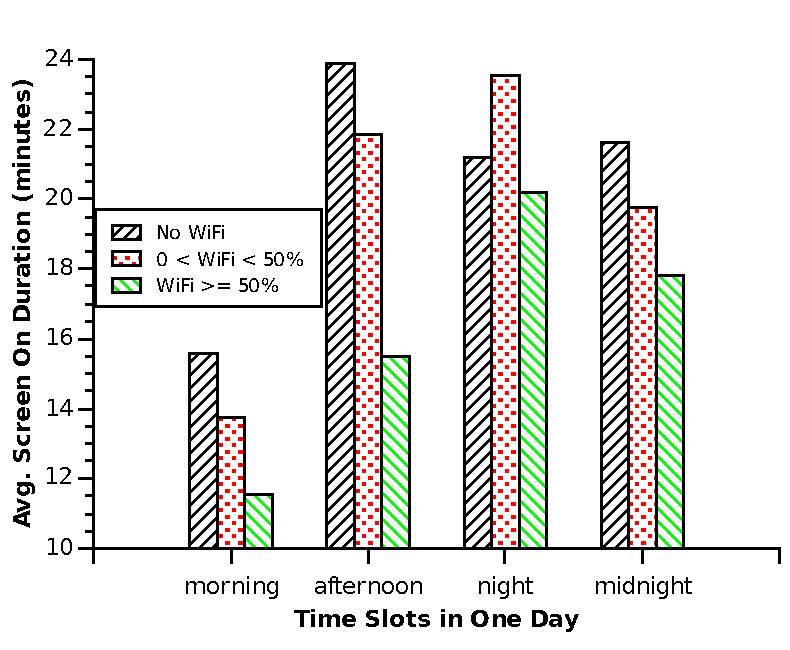
\includegraphics[width = 3.5in]{graphs/dn2.pdf}
\caption{Avg. Screen on Duration in Different Time Slots} 
\label{fig:dn}
\end{figure}

Finally, we explore the relationship of WiFi to 3G usage with respect to various other services on the phone including the number of text
messages, total phone usage, average phone call length, etc. Table~\ref{table:sms_phone} shows the numbers across the entirety of the 
study with users categorized again on a weekly basis.  While WiFi dominant users tended to use their screen for longer
average periods of time, they tended to less frequently use text messages relative to the non-WiFi-dominant users (455 average text messages sent/received per week versus 522 average text messages sent/received per week). Text messages do not count against the data count for either 3G or WiFi usage.  

\begin{table}[h!tbp] 
\caption{WEEKLY SMS/PHONE CALL COMPARISON} 
\label{table:sms_phone}
\centering 
\begin{tabular}{|l|c|c|c|}
\hline
Groups & No WiFi& 0 $<$ WiFi $<$ 50\% & WiFi $>=$ 50\%\\
\hline Avg. Screen On Duration (seconds) & 39.33 & 43.93 & 48.76\\
\hline Avg. SMS All& 436 & 522 & 455  \\ 
\hline Avg. SMS Sent & 209 & 249 & 225 \\
\hline Avg. Number of Phone Calls & 26 & 31 & 24 \\
\hline Avg. Phone Call Duration (hours) & 1.03 & 1.60 & 1.27 \\
\hline Avg. Email All & 89 & 95 & 90\\
\hline Avg. Number of Browser Sessions & 102 & 81 & 67\\
\hline
\end{tabular}
\end{table}

\subsection{App Usage}\label{app}

The network bandwidth and throughput has a profound influence on application usage preference. When the network provides better service,
users tend to use more intensive services.   We look into the data of installed application and application traffic which are logged by the service as part of the agent (hourly application data usage). 

\begin{table}[h!tbp] 
\caption{TOP APPLICATIONS CATEGORIES} 
\label{table:app_categories}
\centering 
\begin{tabular}{|l|c|c|c|}
\hline
& No WiFi & 0 $<$ WiFi $<$ 50\% & WiFi $>=$ 50\%\\
\hline
Top Downlink & Browser & Browser & Netflix\\ 
					& Facebook & Facebook & Browser\\
					& Zynga Words & Pandora & Pandora\\
					& Amazon & Zynga Words & Facebook\\
					& Twitter & Twitter & Dictionary\\
\hline
Top uplink & Google Maps & Google Maps & Pandora\\ 
					& PhoneMonitor & Pandora & Google Maps\\
					& Browser & PhoneMonitor & Glu Games\\
					& Facebook &Browser&PhoneMonitor\\
					& Gmail & Facebook&Browser\\
\hline
\end{tabular}
\end{table}


In Table~\ref{table:app_categories} we summarize the top 5 applications appeared in the each group based on their total downlink or uplink traffic. For the phones using WiFi more than 50\%, streaming apps such as Netflix and Pandora always are the top applications. For the participants using 3G only, their main activities on the phone are web browsing and email checking. Figure~\ref{fig:app_downlink} demonstrates the weekly downlink traffic of the top 10 apps in different categories which include video \& audio (Netflix, Youtube, Pandora and Google Music), social (Facebook and Twitter), tools (Browser, Gmail, Google Maps, Dictionary) and games (Zynga and Glu applications). Similarly, we present the results of uplink traffic in Figure~\ref{fig:app_uplink}. In both graphs, the traffic of video and audio applications increases dramatically when the participants use more WiFi. An interesting
question emerges if the streaming consumption is user specific or rather becomes enabled by WiFi speeds
implying that WiFi with continuous LTE would show the same usage patterns. 

\begin{figure}[h!tbp]
\centering
{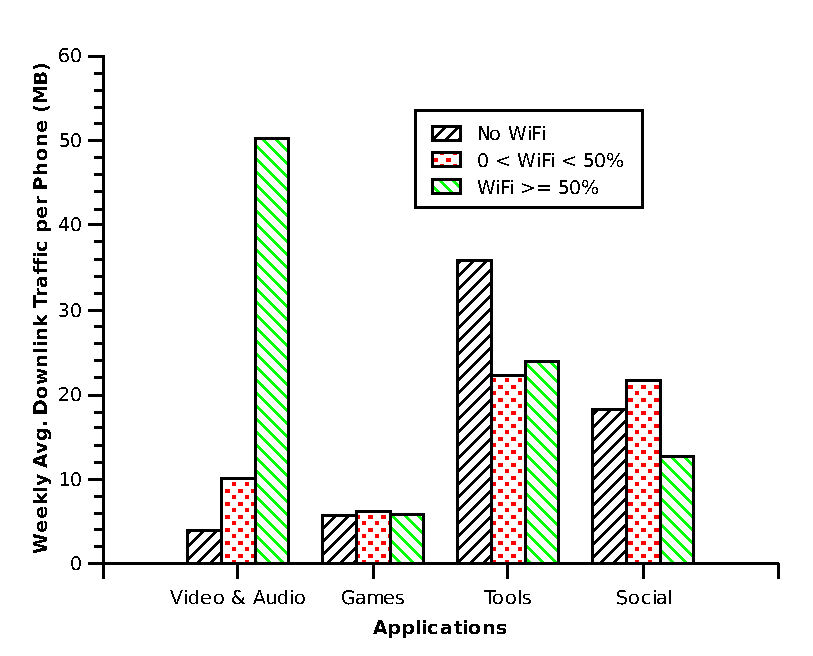
\includegraphics[width = 3.5in]{graphs/app_downlink.pdf}}
\caption{Weekly Application Downlink Traffic} 
\label{fig:app_downlink}
\end{figure}

\begin{figure}[h!tbp]
\centering
{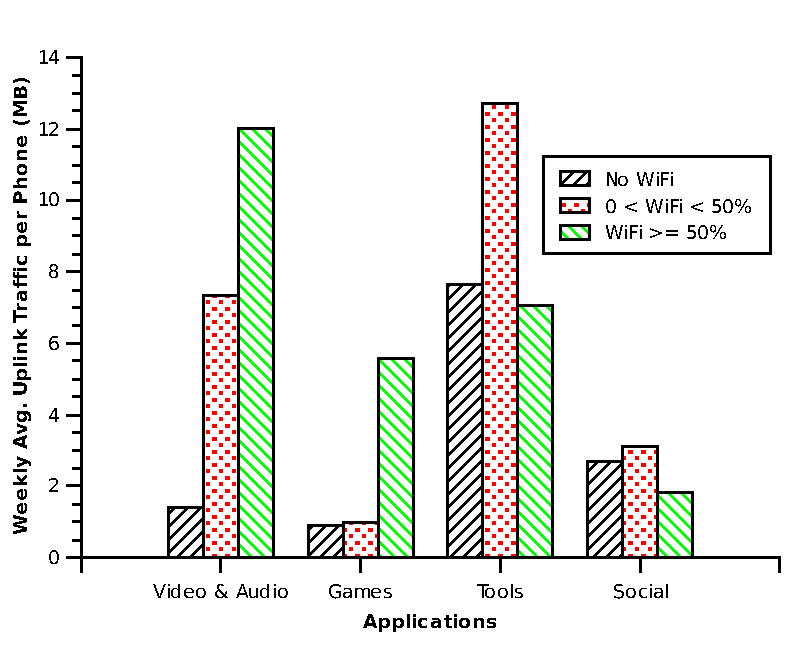
\includegraphics[width = 3.5in]{graphs/app_uplink.pdf}}
\caption{Weekly Application Uplink Traffic} 
\label{fig:app_uplink}
\end{figure}

\section{Summary}
To that end, we make the following contributions in this chapter:
\begin{itemize}
\item The net result of our findings over an eight week period of our smartphone
usage data shows that the gaps in WiFi coverage for smartphones temper the perceived potential gains by 
WiFi offloading. More attention should be paid to WiFi coverage to examine said coverage through the
lens of a typical smartphone rather than a typical laptop or tablet device. 

\item We explore the relationship of WiFi data consumption and phone usage time deduced by screen session length. Moreover,
our work includes accommodations for considering SMS/phone call/browser impacts with regards to phone usage.

\end{itemize}
Although individual handsets (ex. iPhone) may possess better WiFi characteristics, the heterogeneity
of available handsets implies that it is exceptionally likely there will significant variations in the ability of phones to
take advantage of WiFi offloading. While certainly any offloading is desperately appreciated due to capacity
shortages, WiFi offloading may be further clouded by bottlenecks in the next hop following the WiFi link as well. Therefore, we believe that additional scrutiny is needed with respect to the end benefits that can arise from WiFi offloading. In next chapter, we discuss the potential of opportunistic relaying which is complementary to WiFi offloading and demonstrate that the concept of opportunistic networks is powerful in face of data tsunami. 
